\chapter{Duality}

\clearpage
\section{The Lagrange dual function}

\clearpage
\section{The Lagrange dual problem}

\clearpage
\section{Geometric interpretation}

\clearpage
\section{Saddle-point interpretation}

\clearpage
\section{Optimality conditions}

\clearpage
\section{Perturbation and sensitivity analysis}

\clearpage
\section{Examples}

\clearpage
\section{Theorems of alternatives}

\clearpage
\section{Generalized inequalities}


\clearpage
\hfil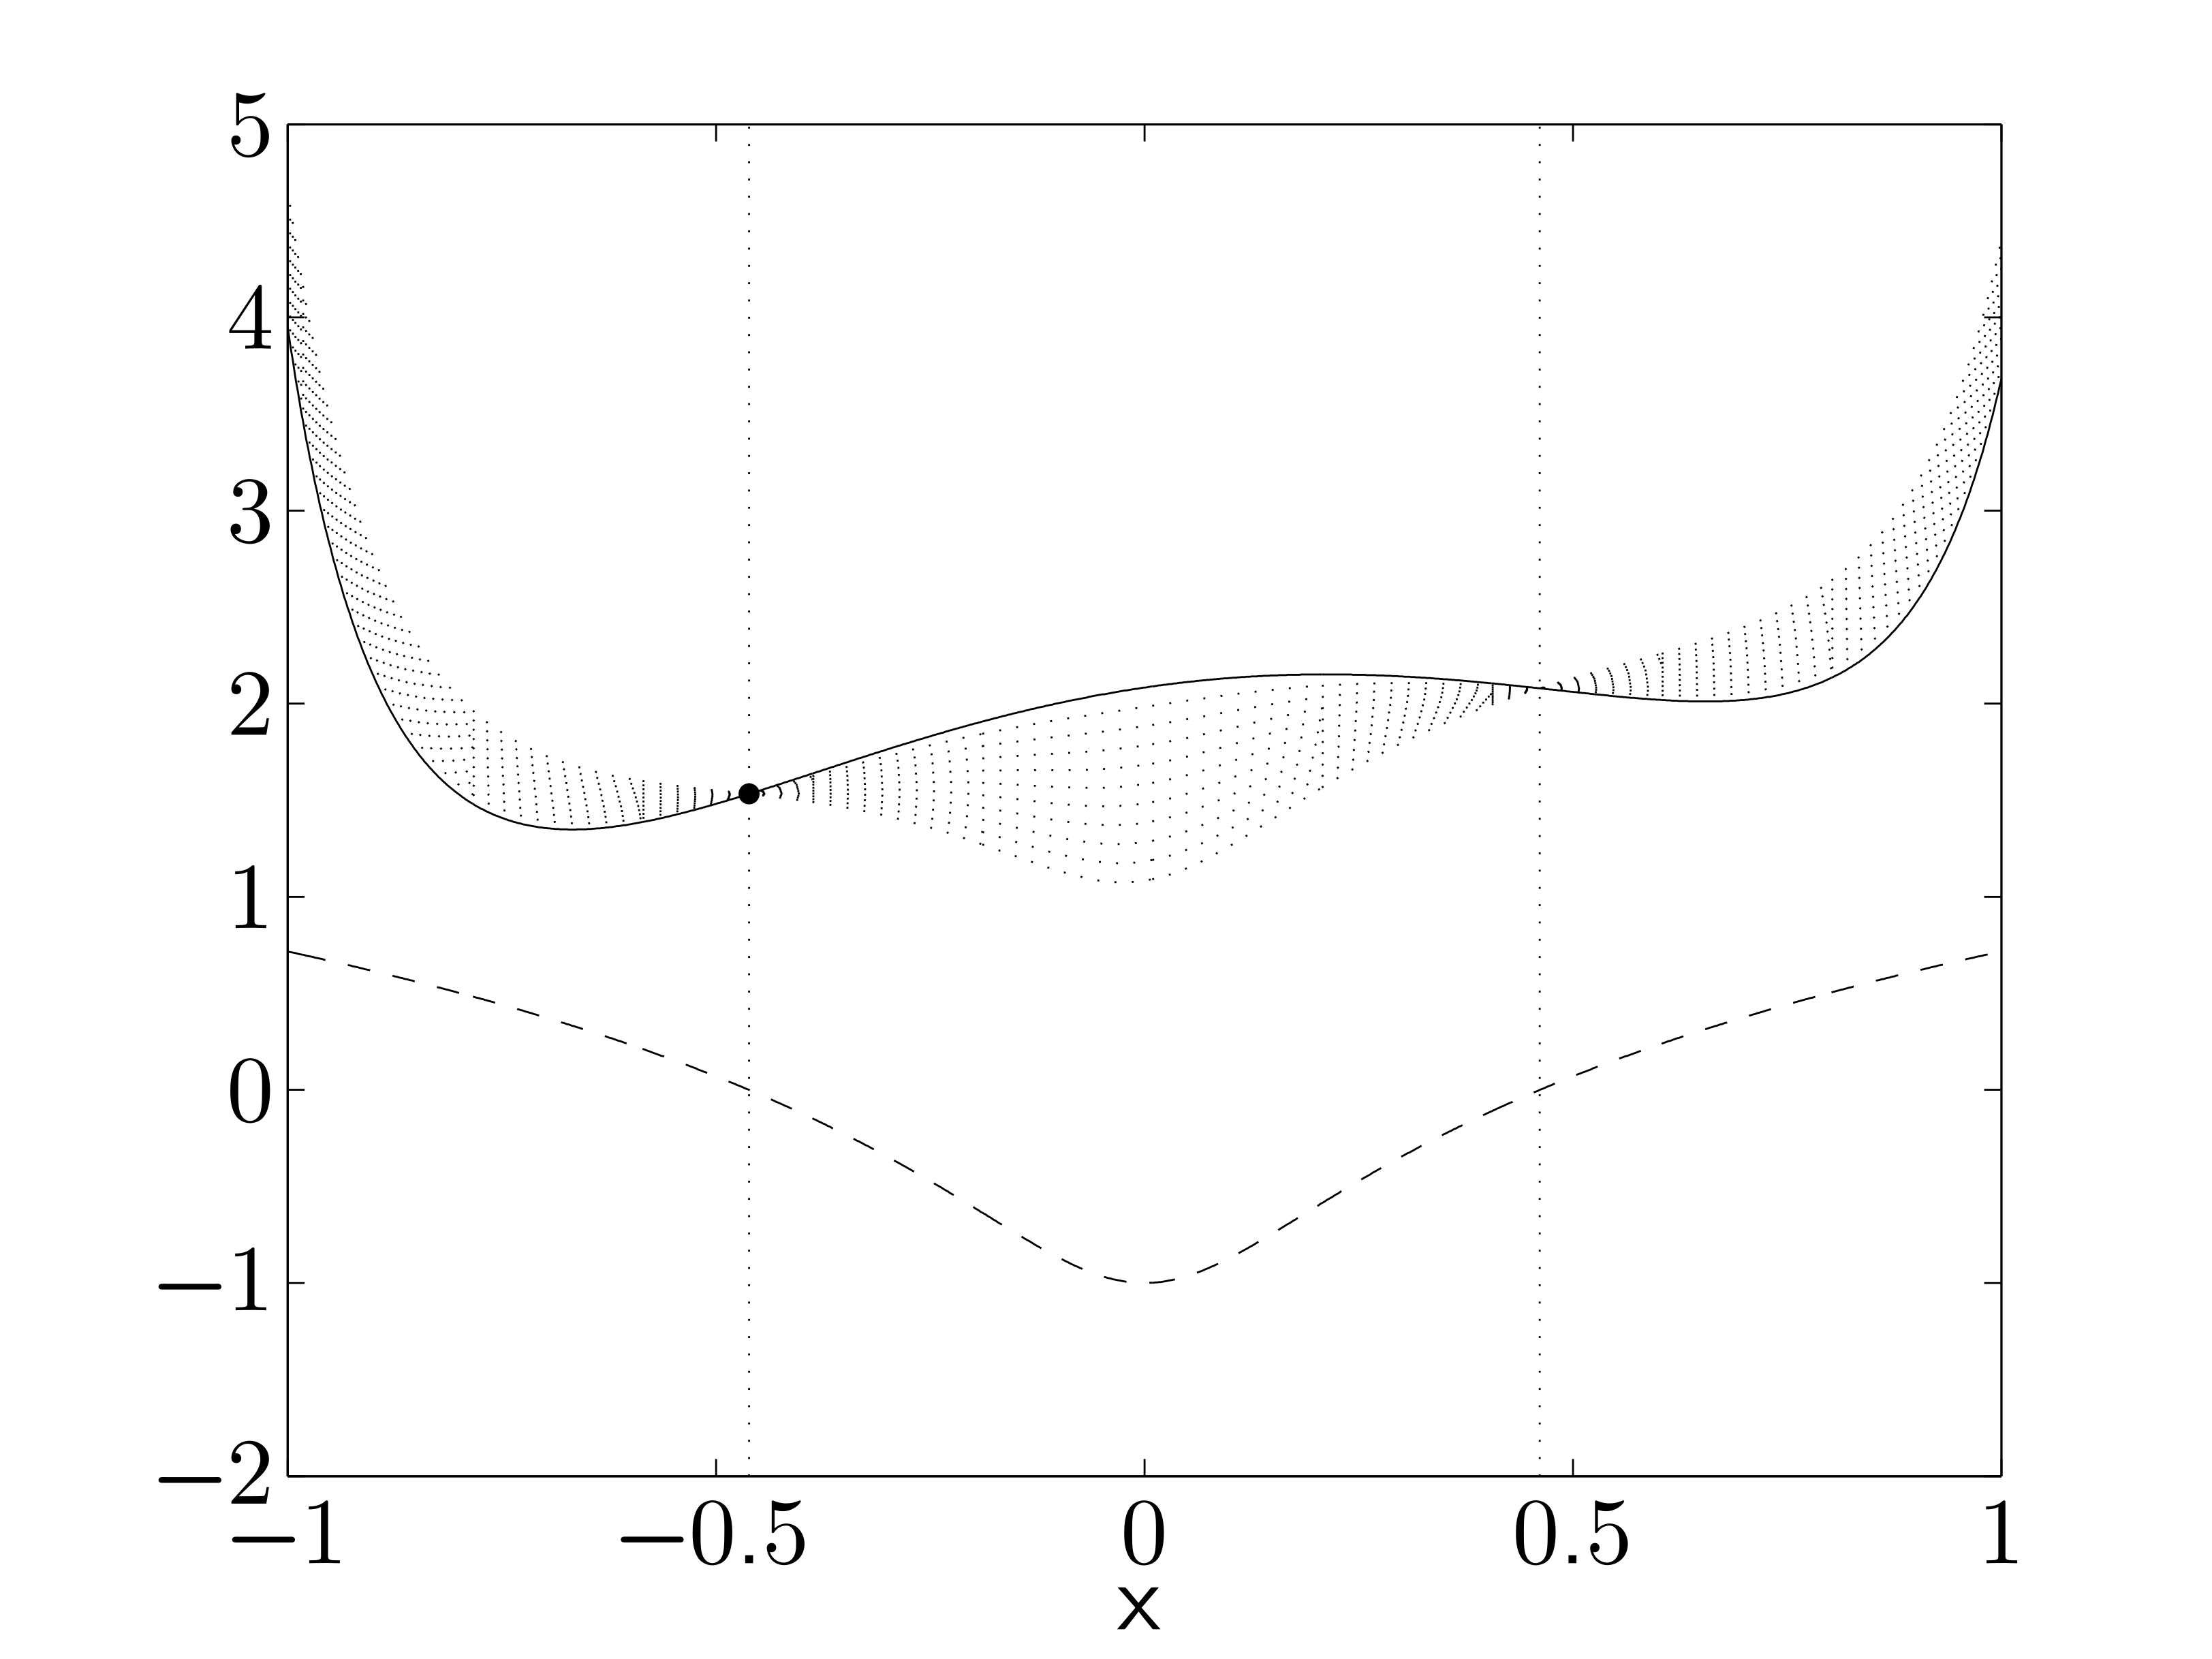
\includegraphics[width=.5\textwidth]{../Graphics/217a.png}\hfil

\clearpage
\hfil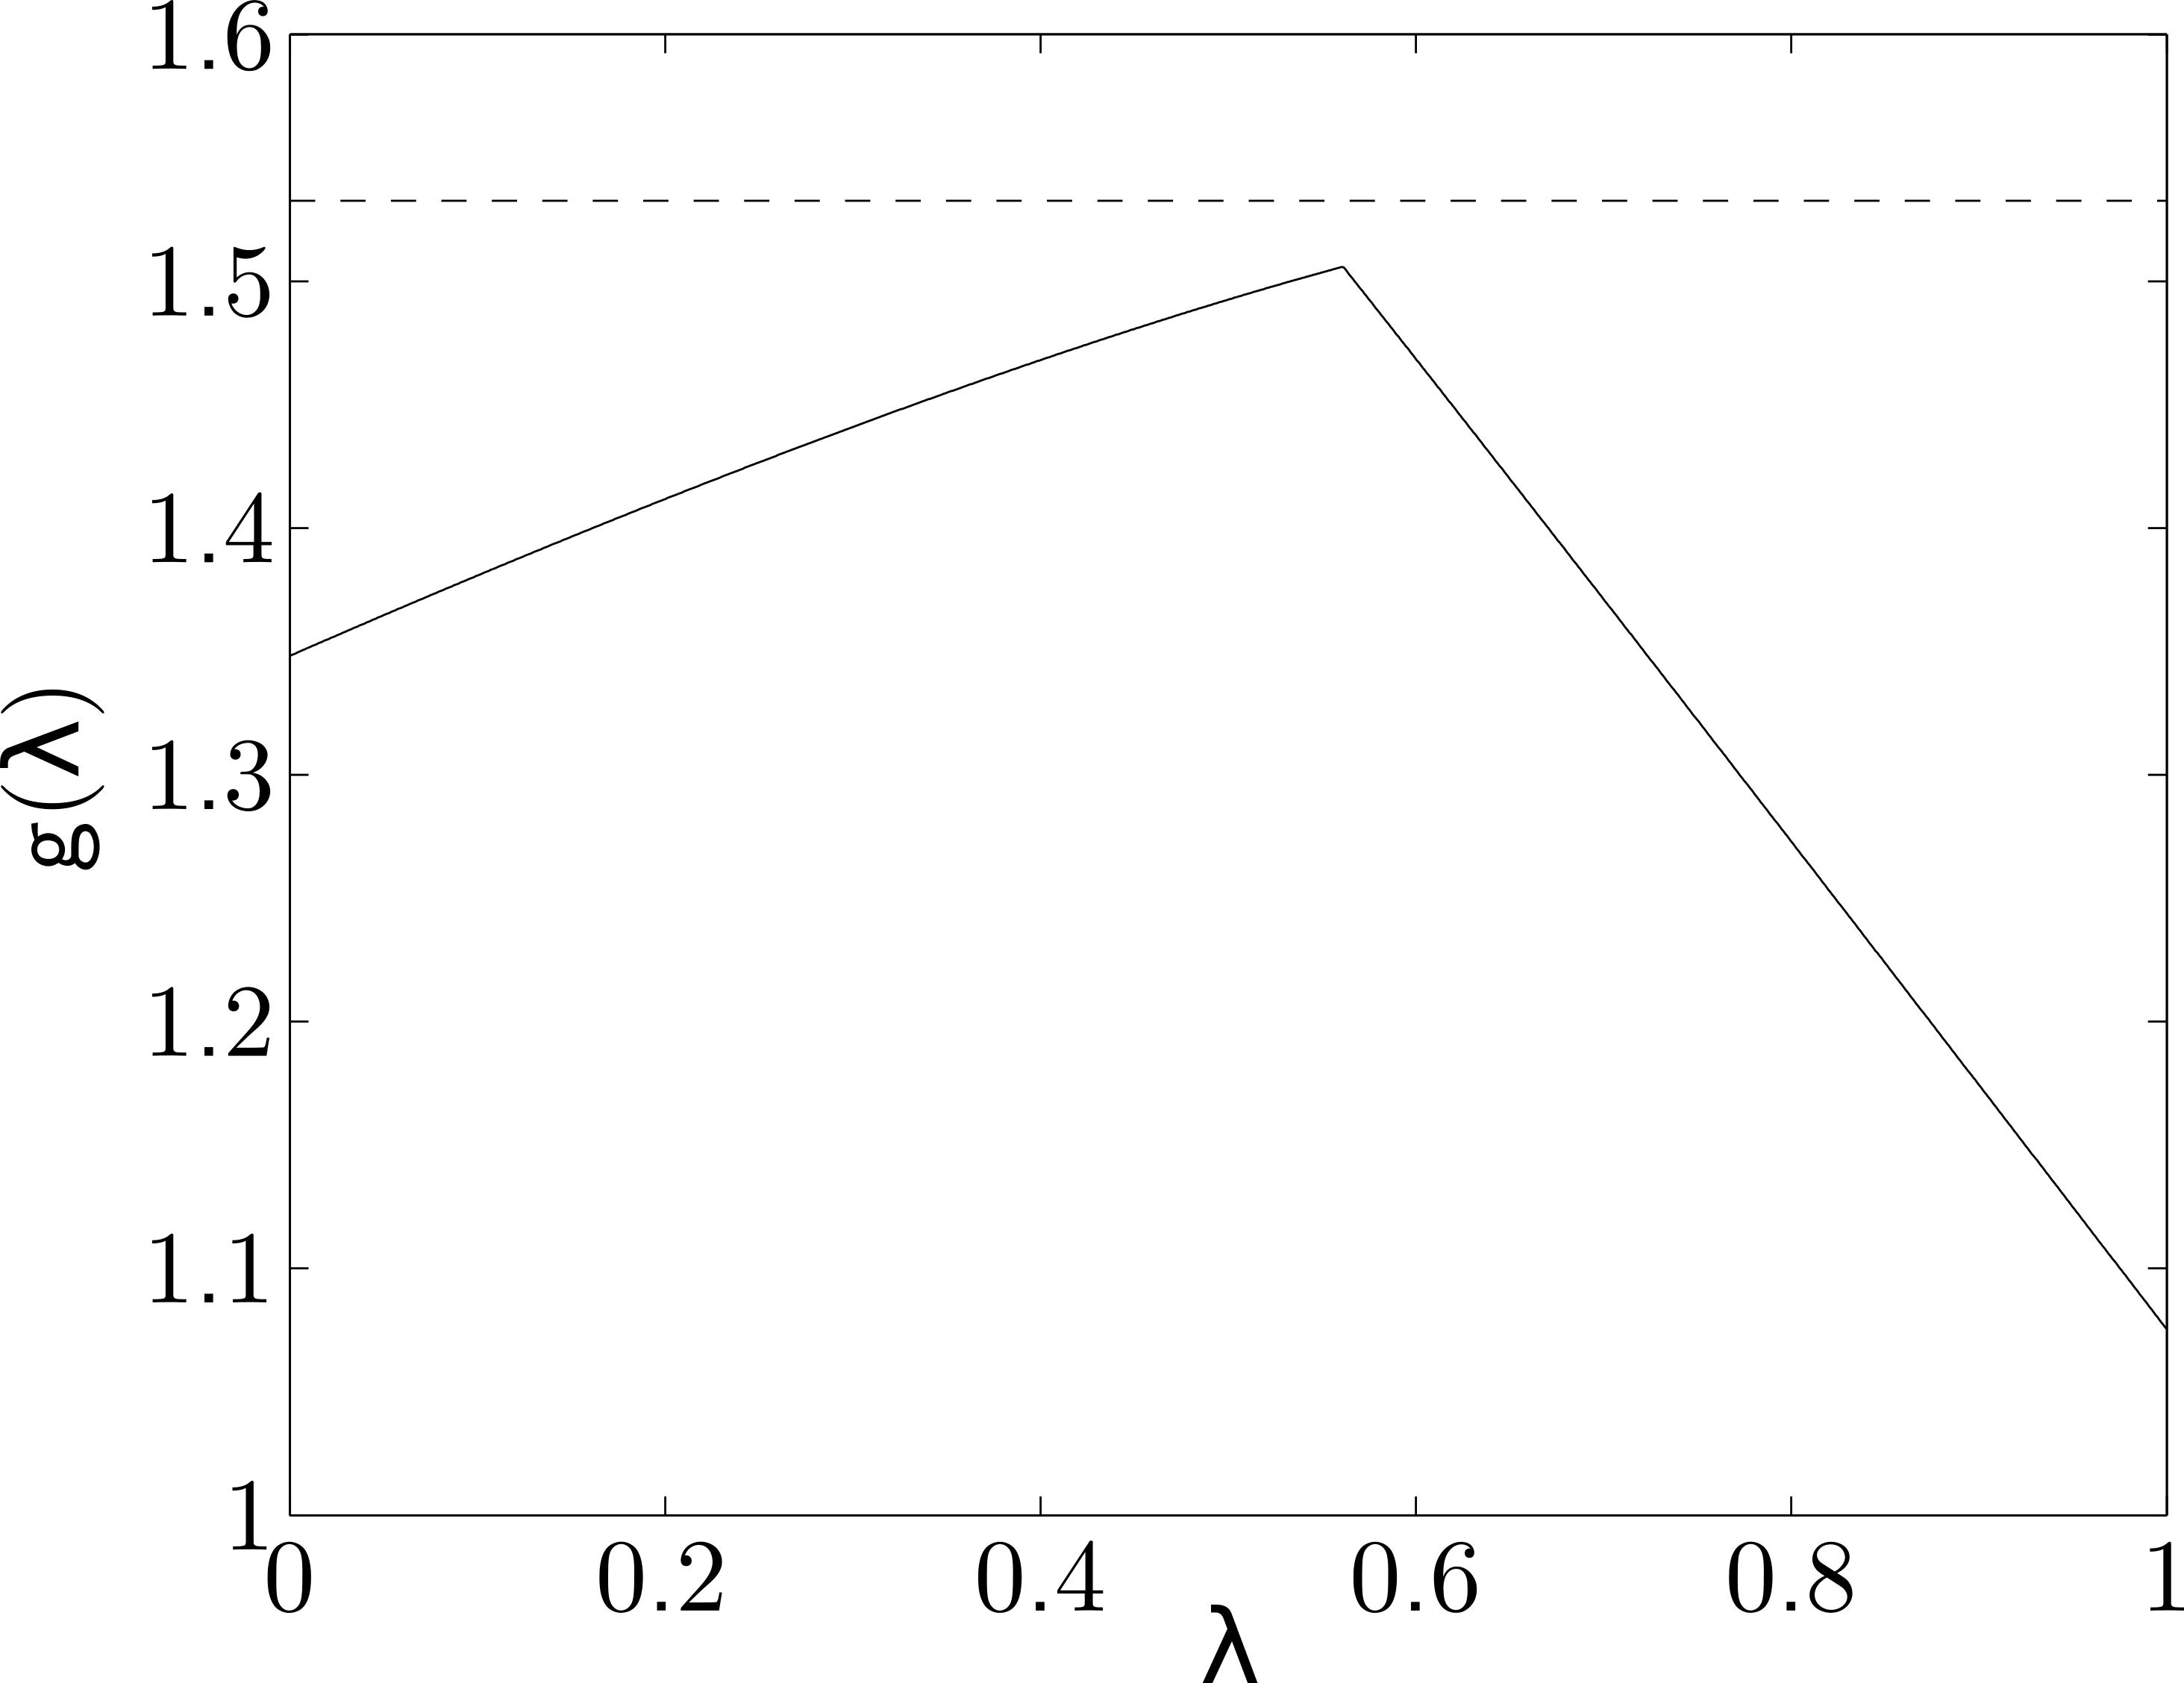
\includegraphics[width=.5\textwidth]{../Graphics/217b.png}\hfil

\clearpage
\hfil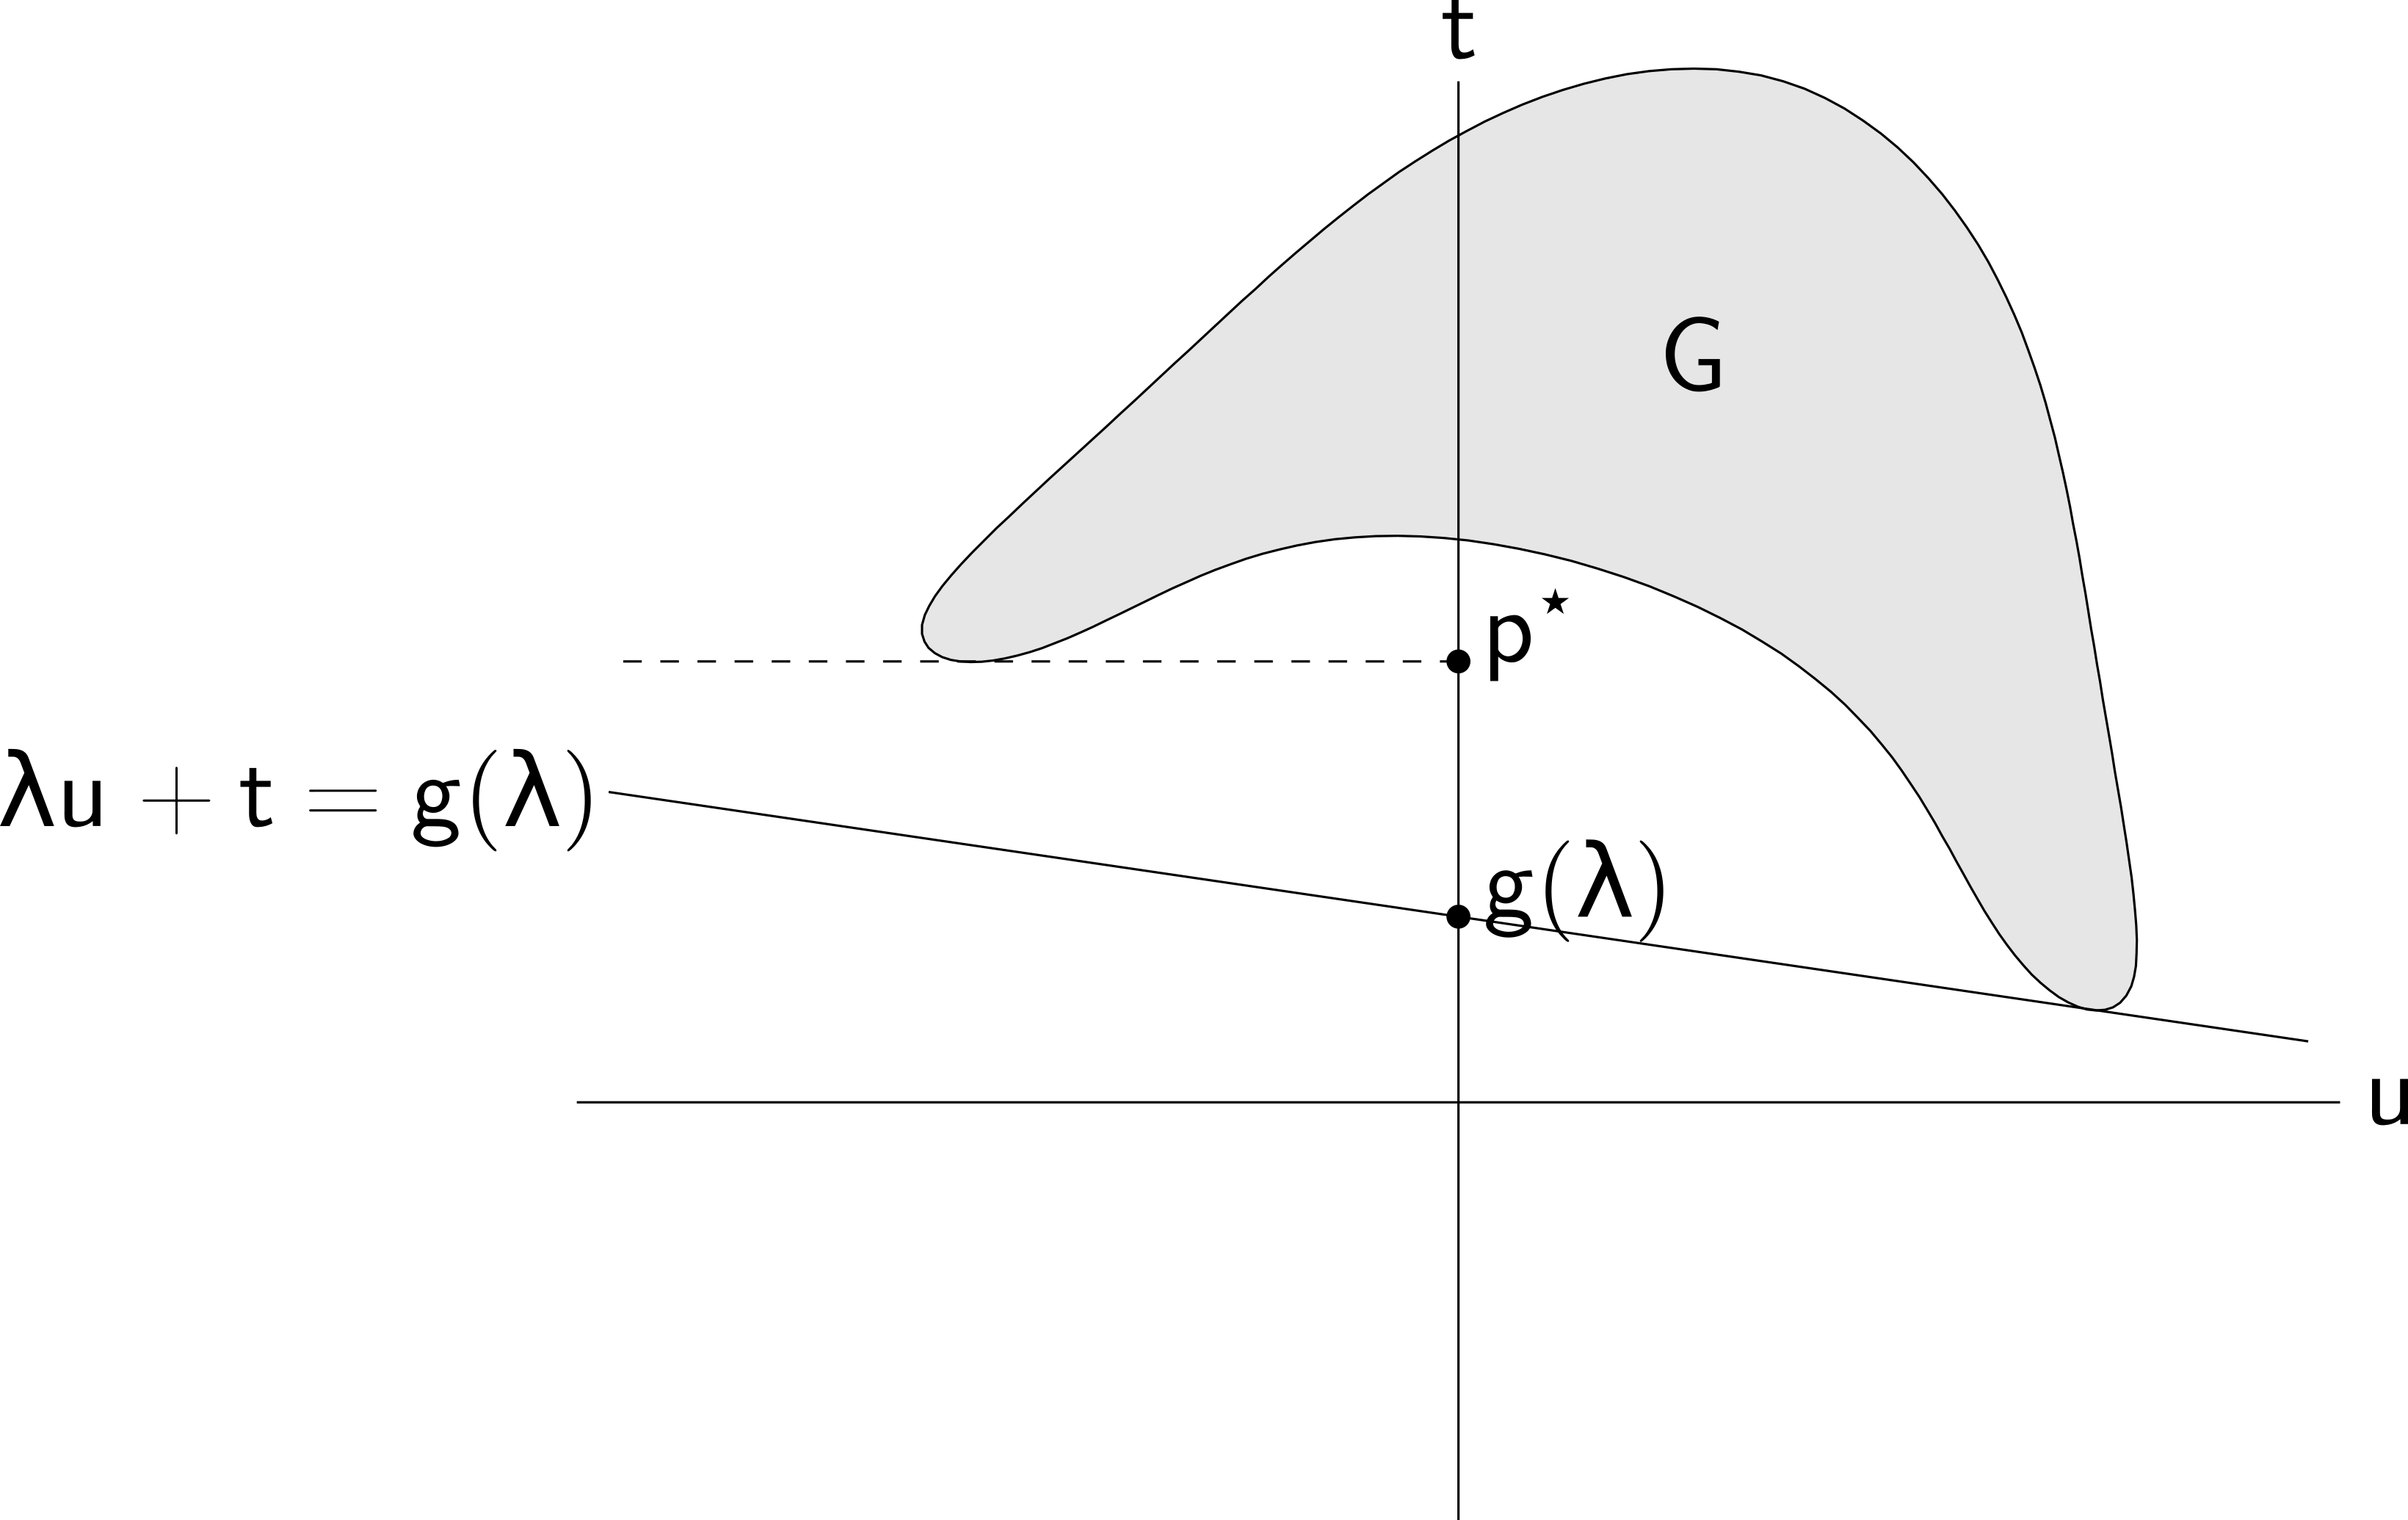
\includegraphics[width=.5\textwidth]{../Graphics/233a.png}\hfil

\clearpage
\hfil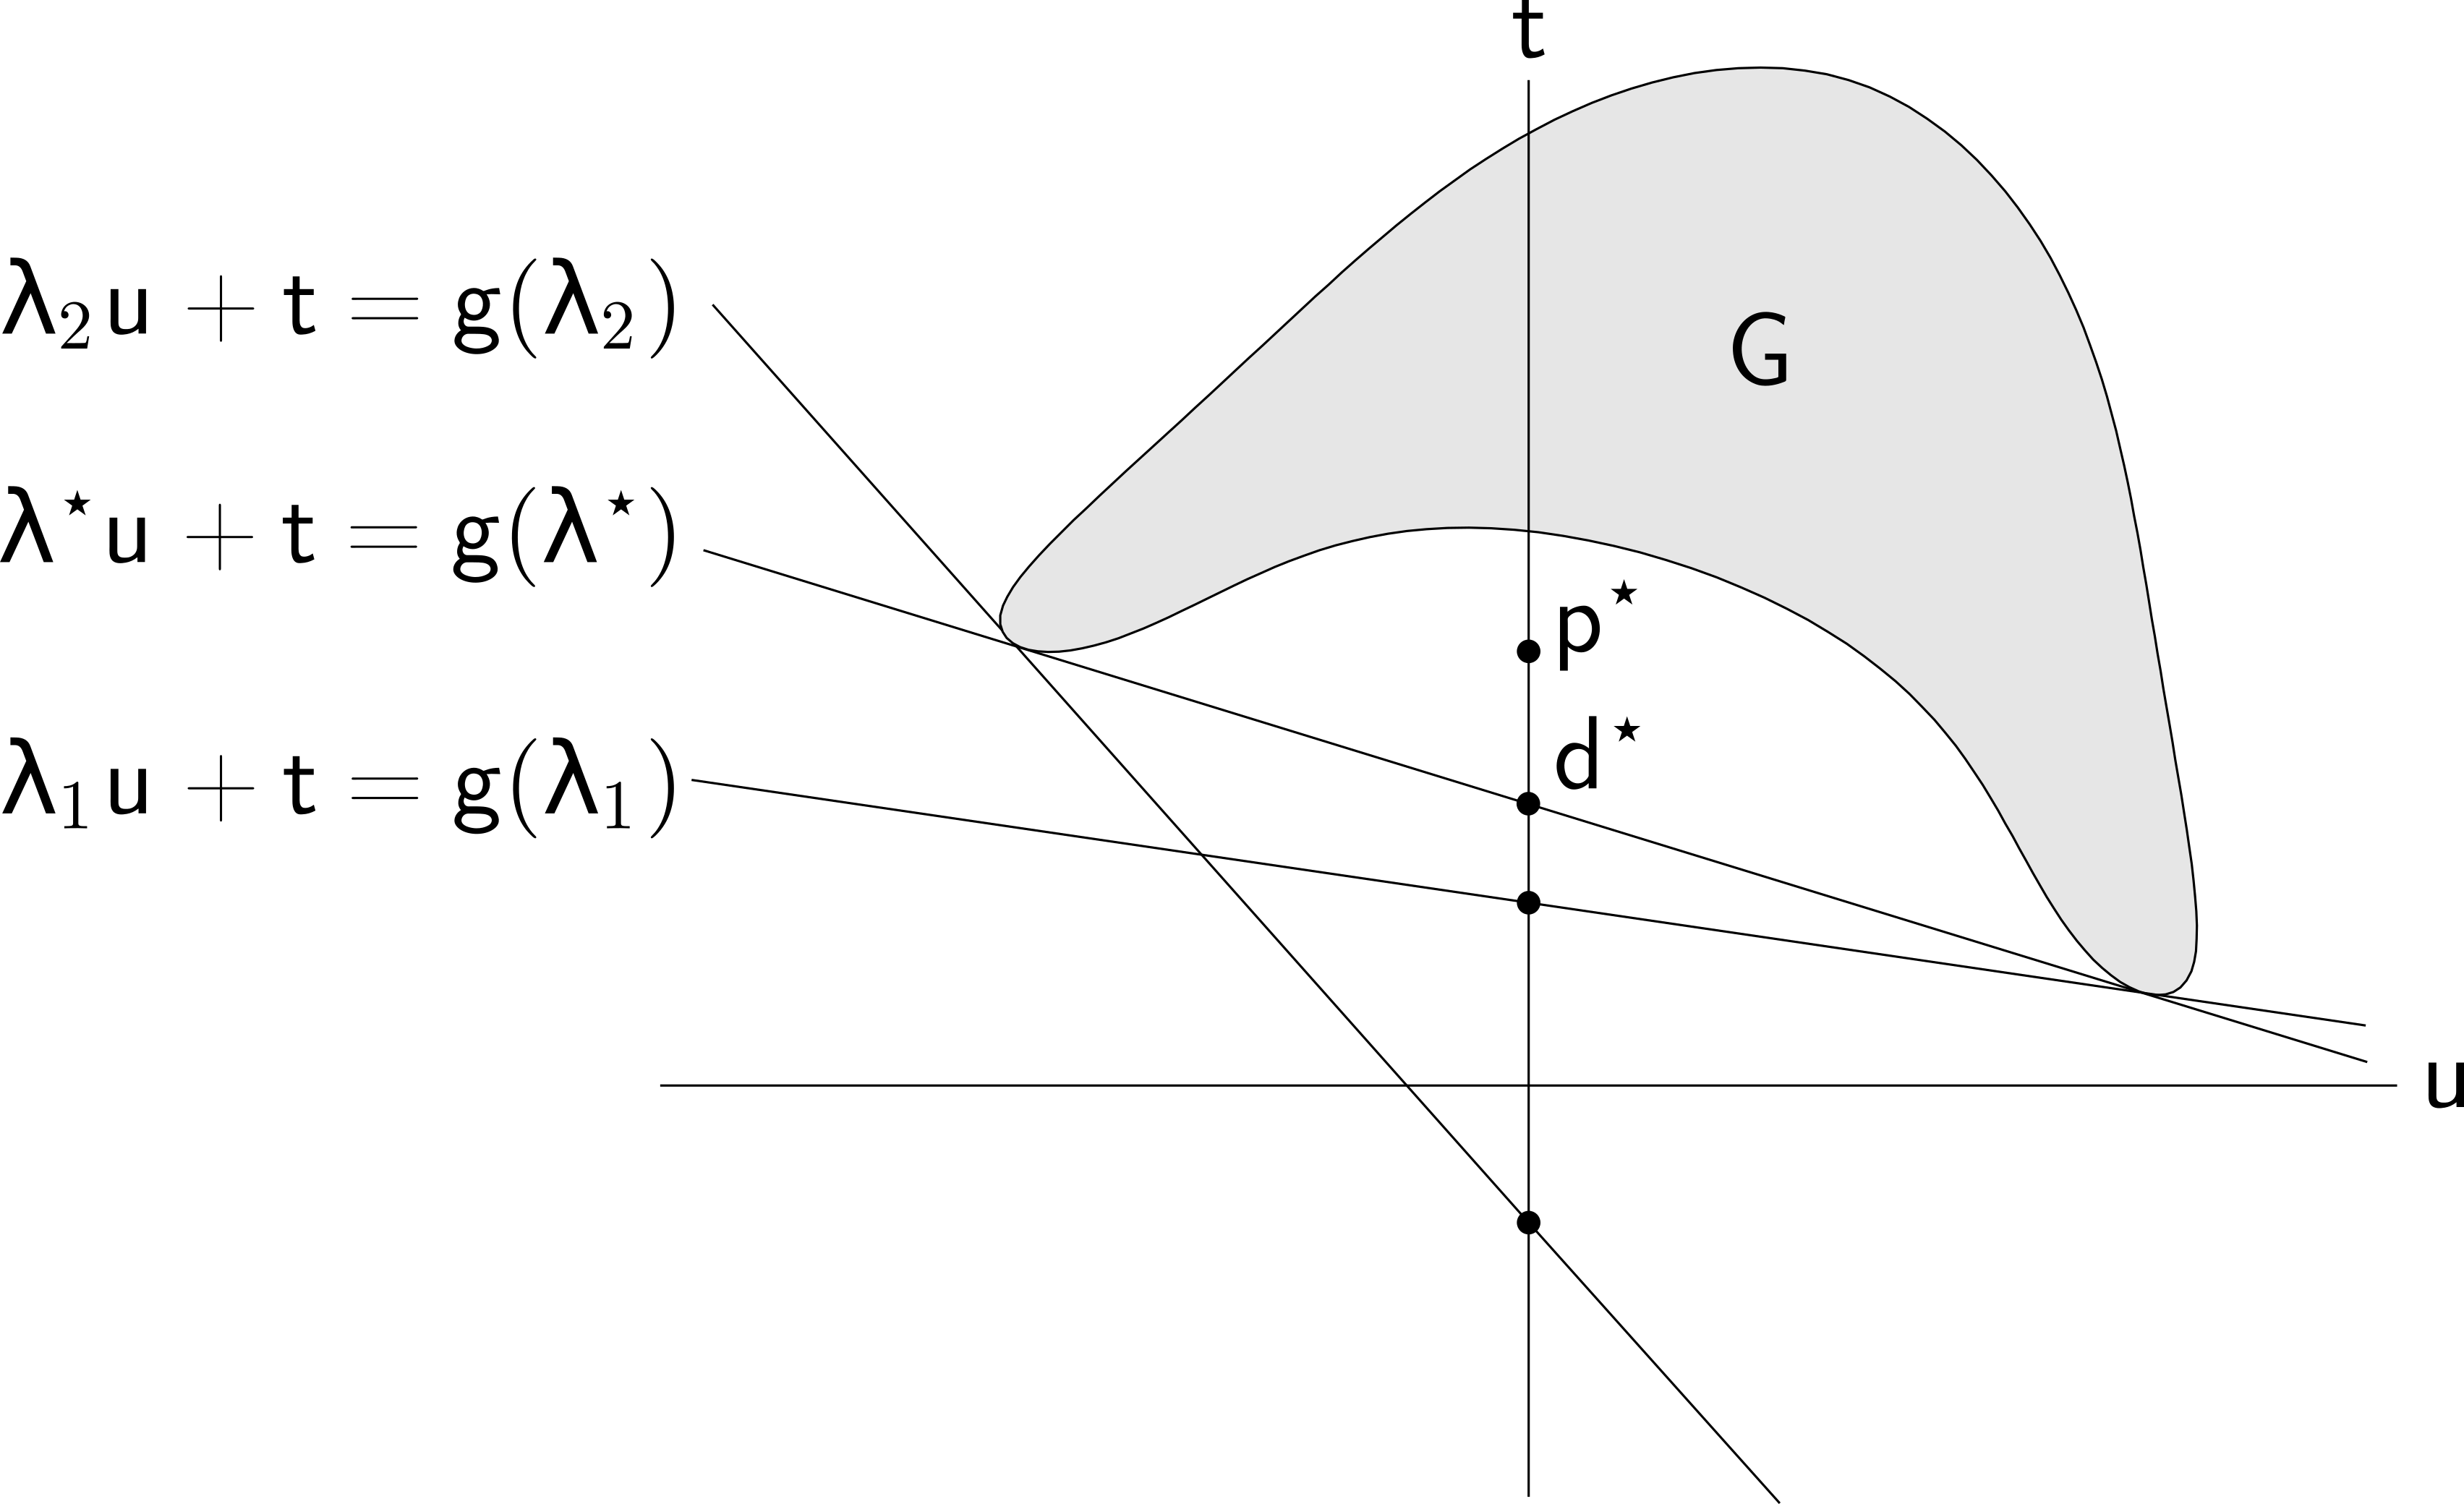
\includegraphics[width=.5\textwidth]{../Graphics/233b.png}\hfil

\clearpage
\hfil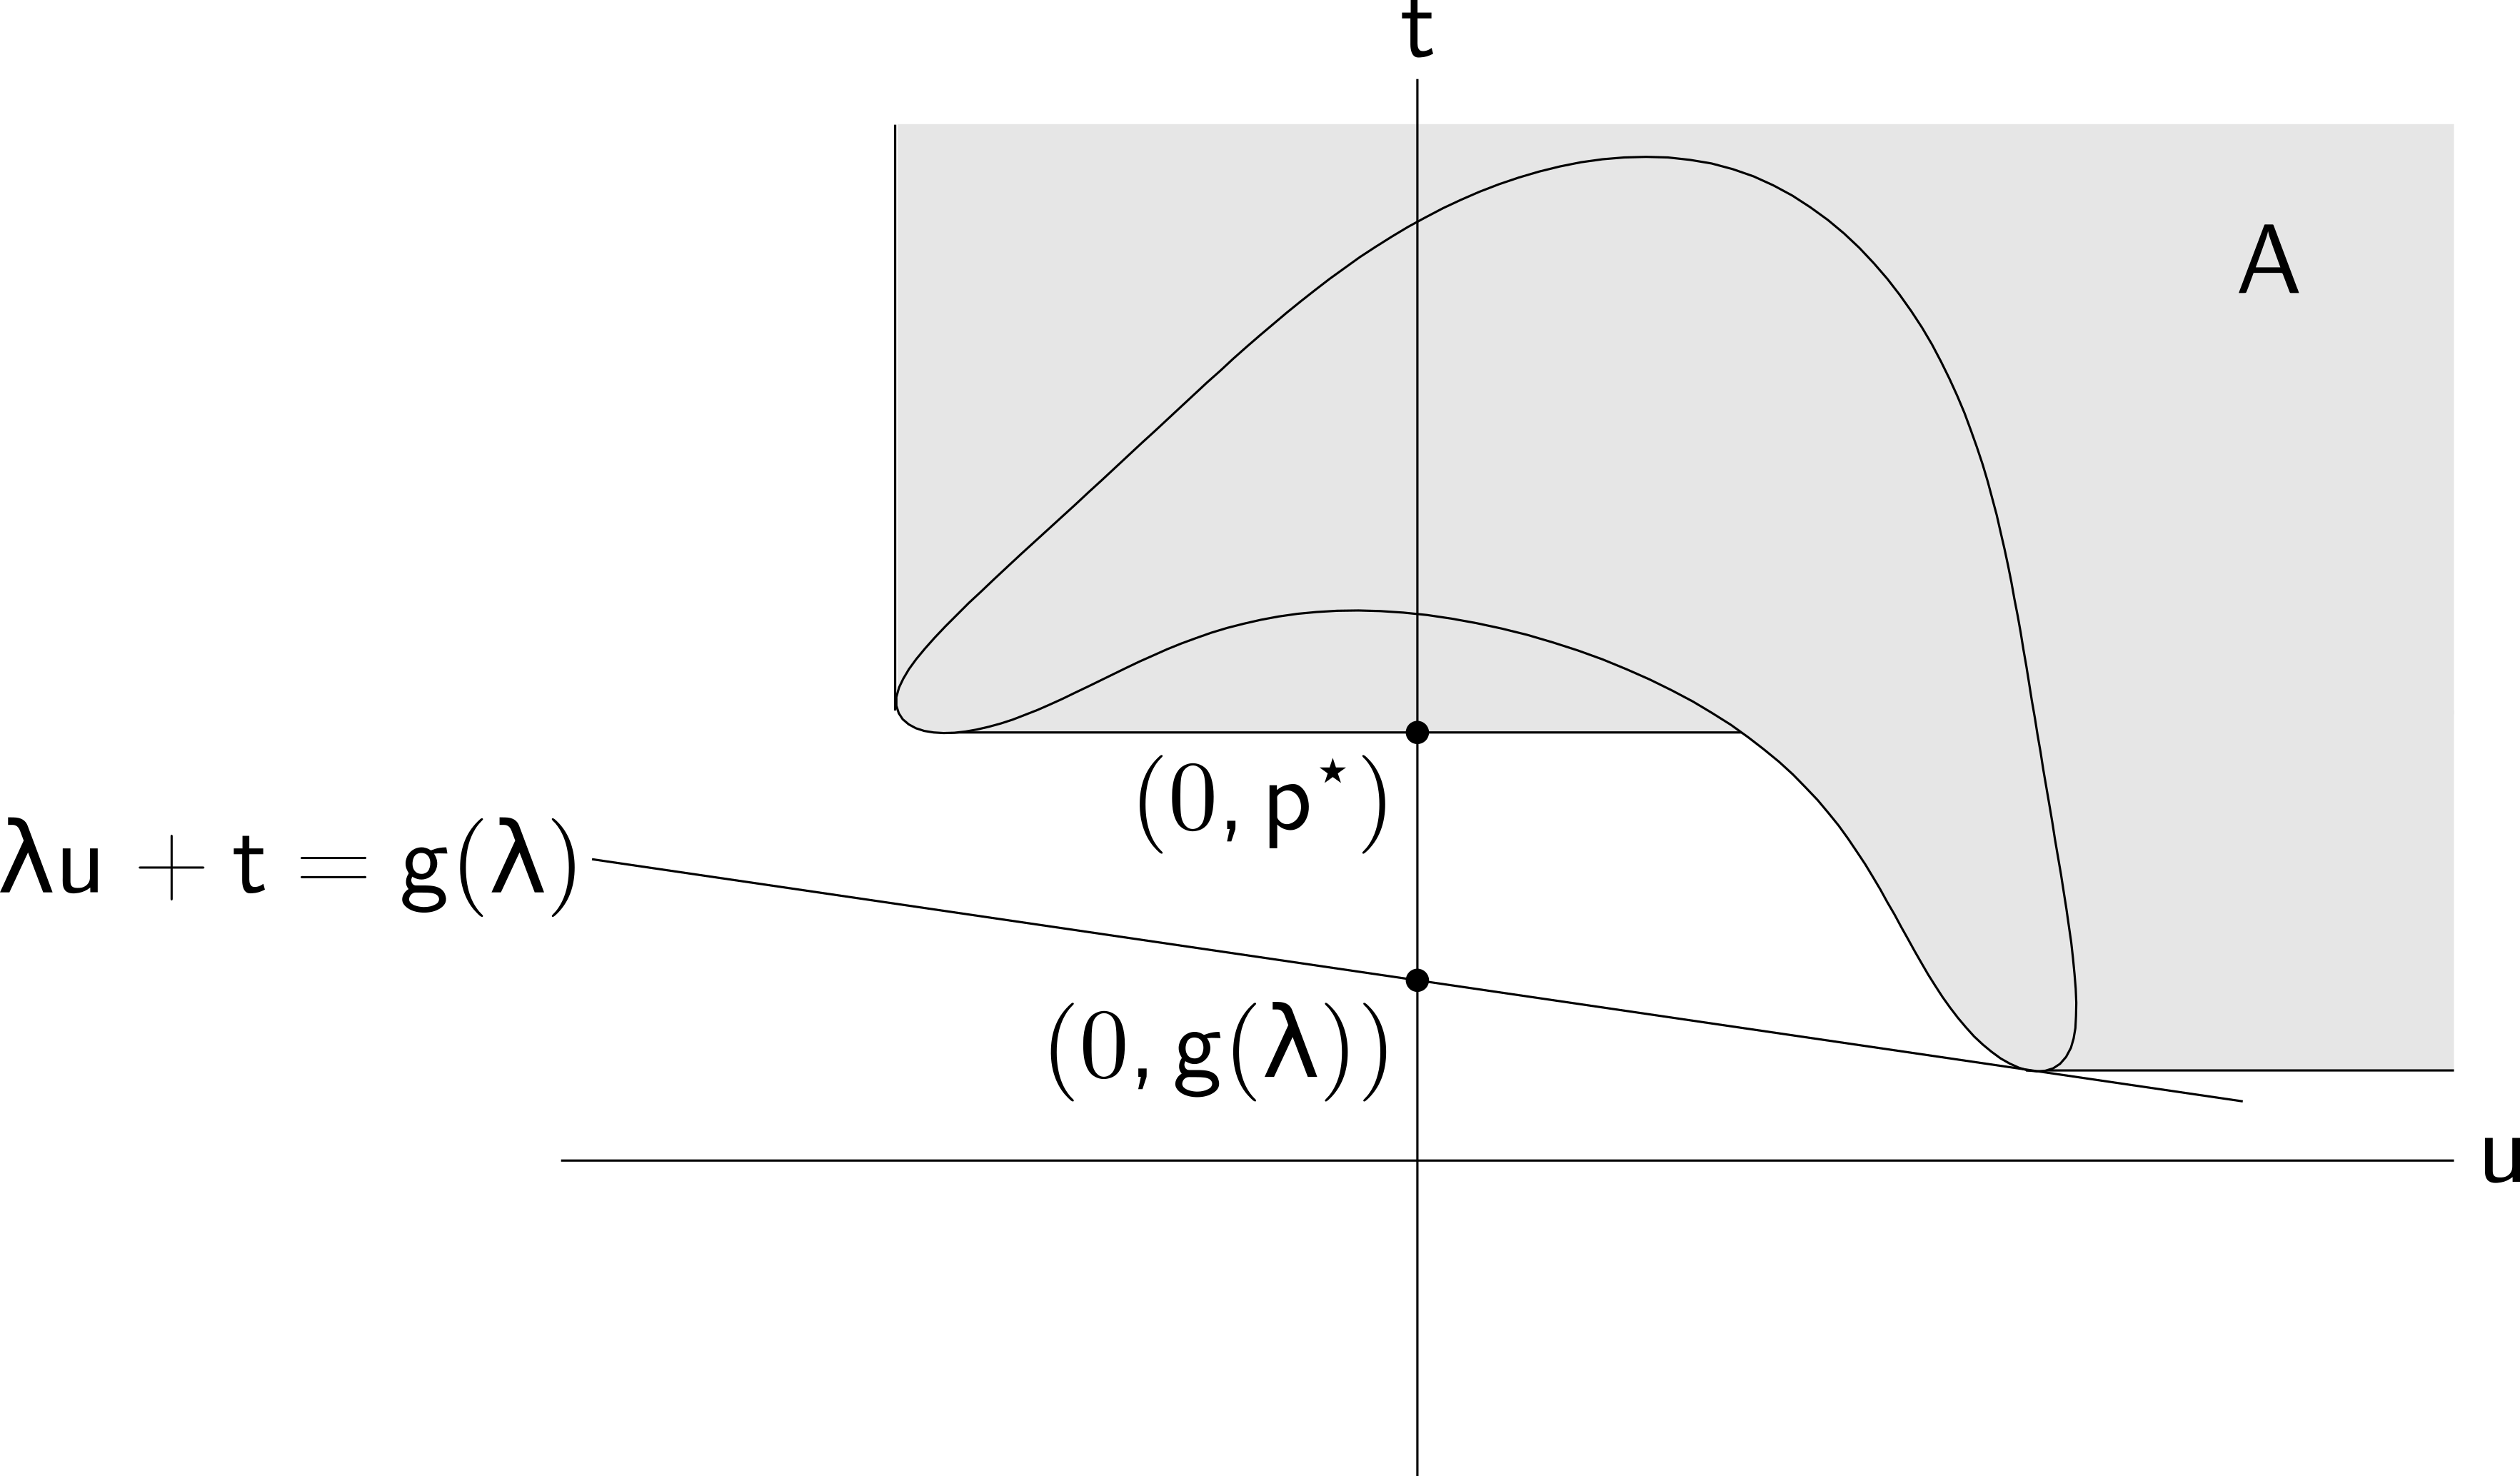
\includegraphics[width=.5\textwidth]{../Graphics/234.png}\hfil

\clearpage
\hfil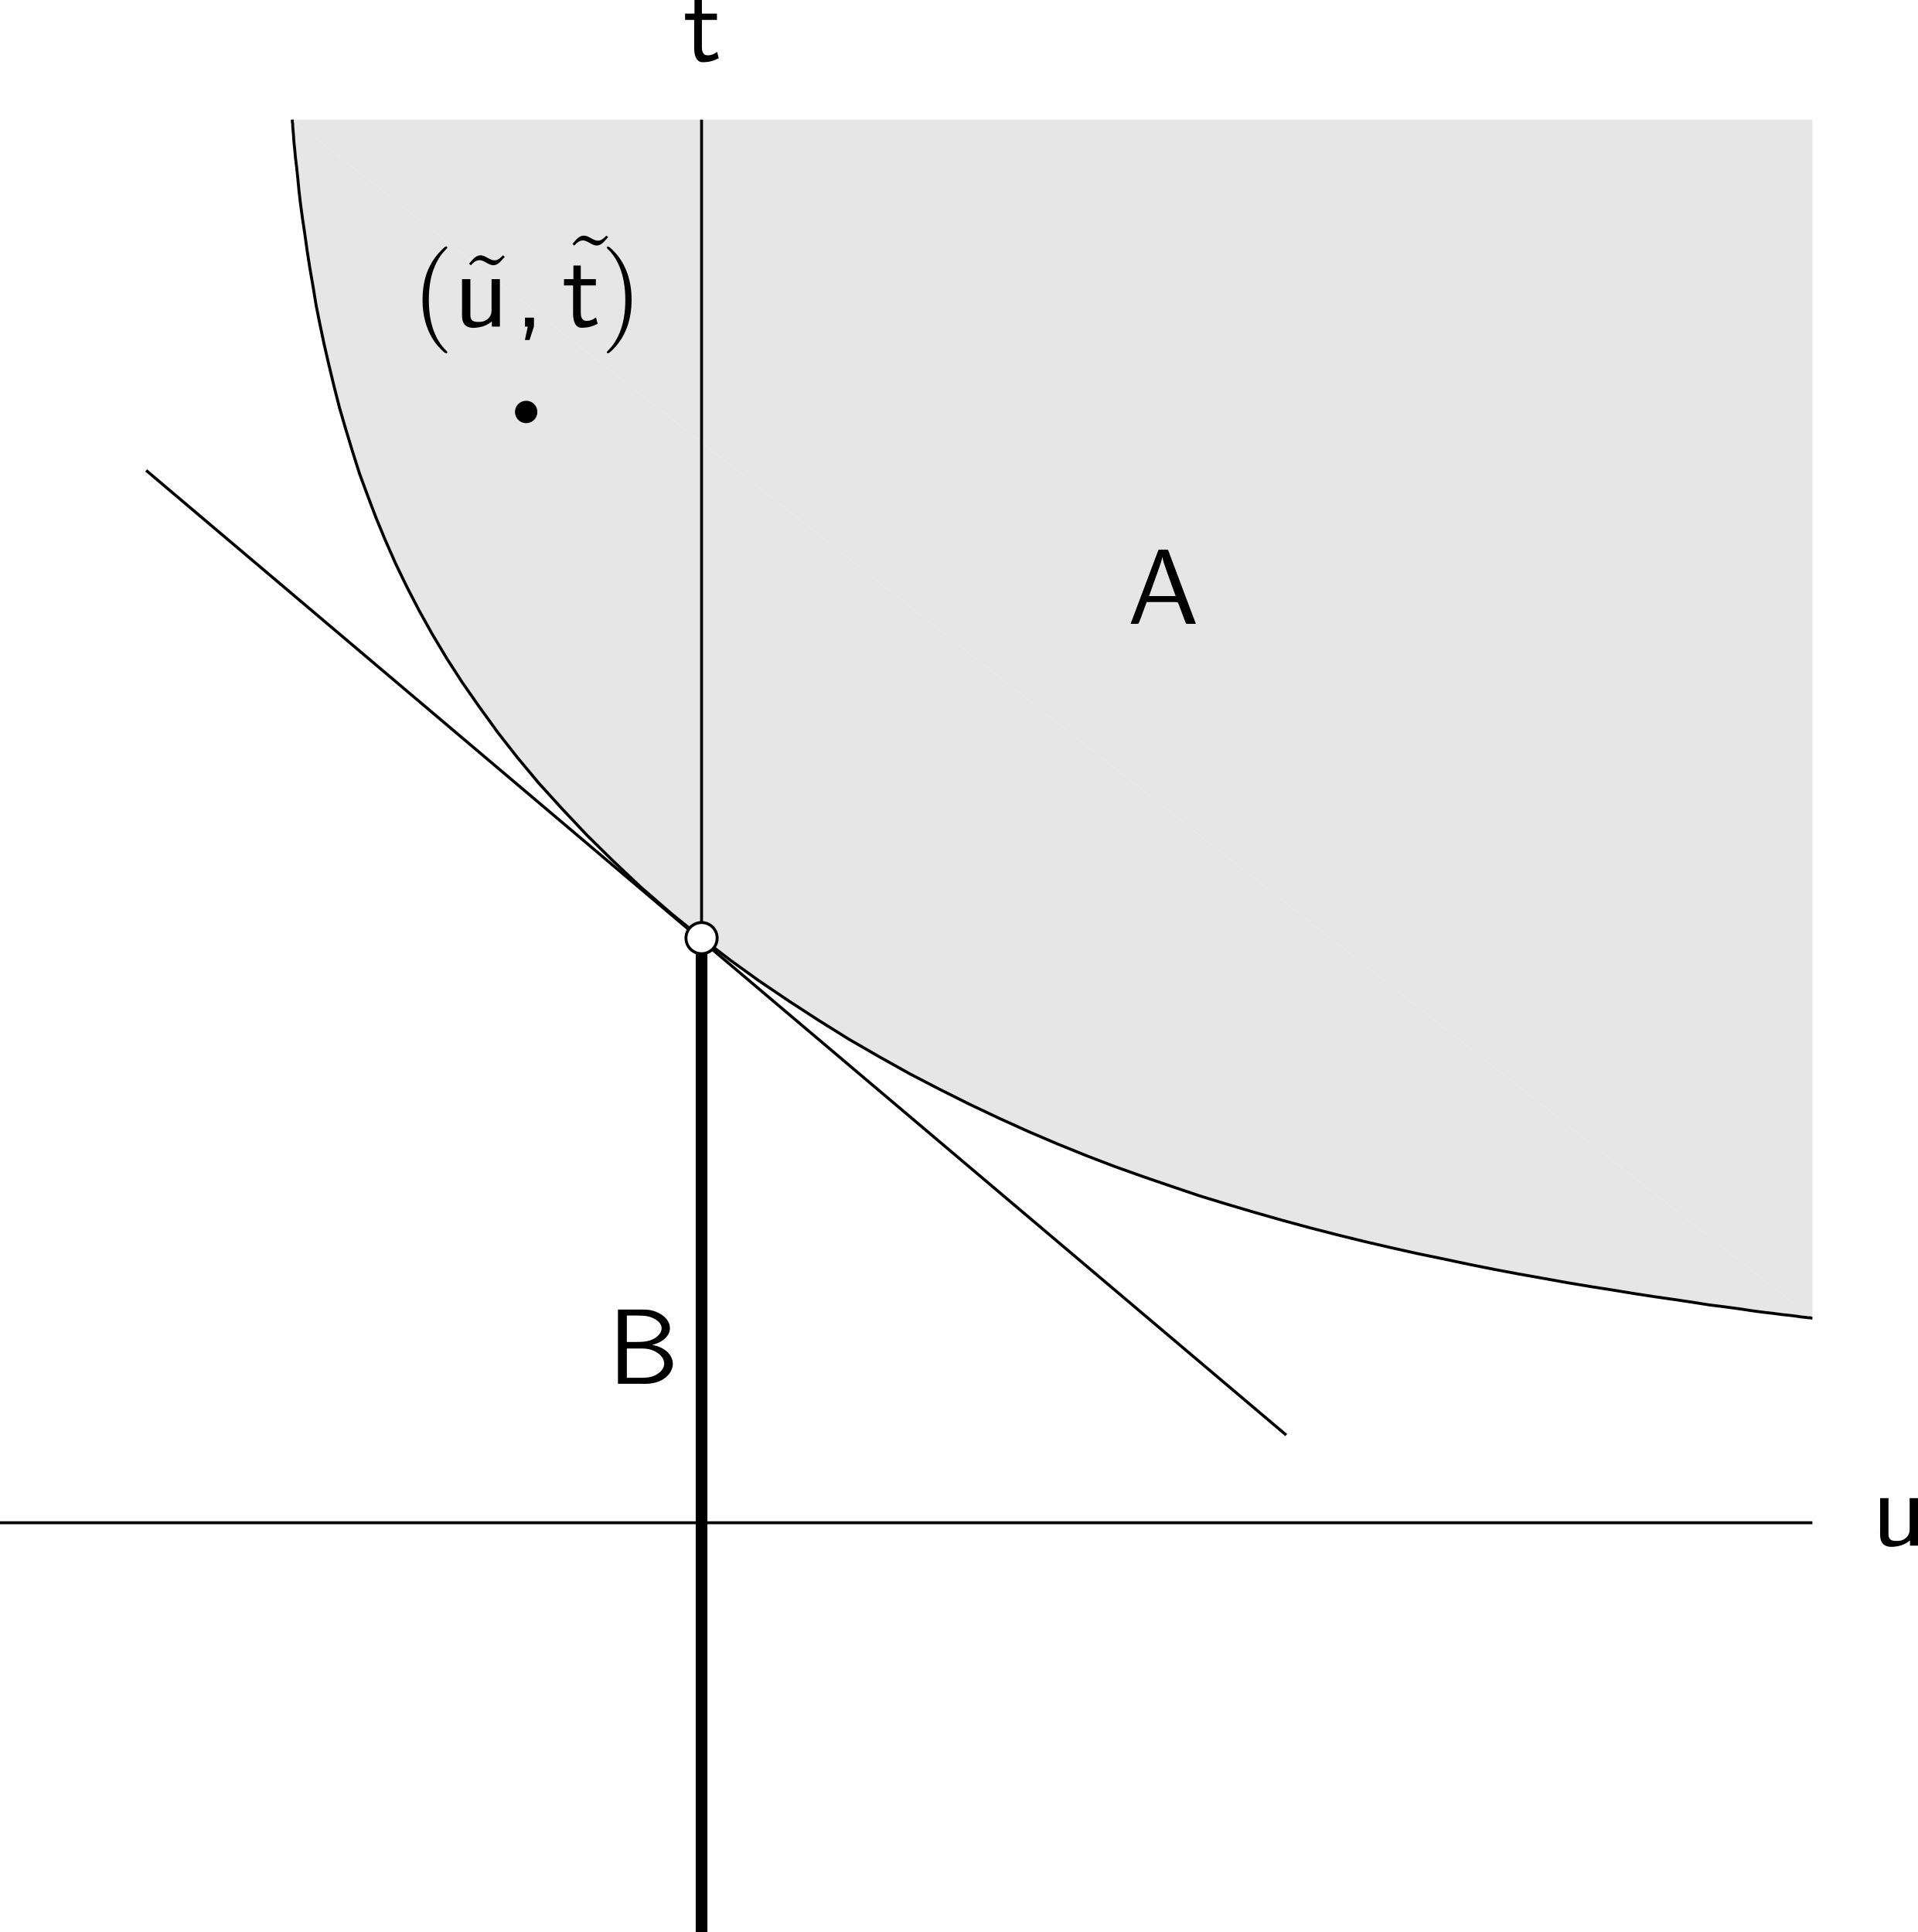
\includegraphics[width=.5\textwidth]{../Graphics/236.png}\hfil

\clearpage
\hfil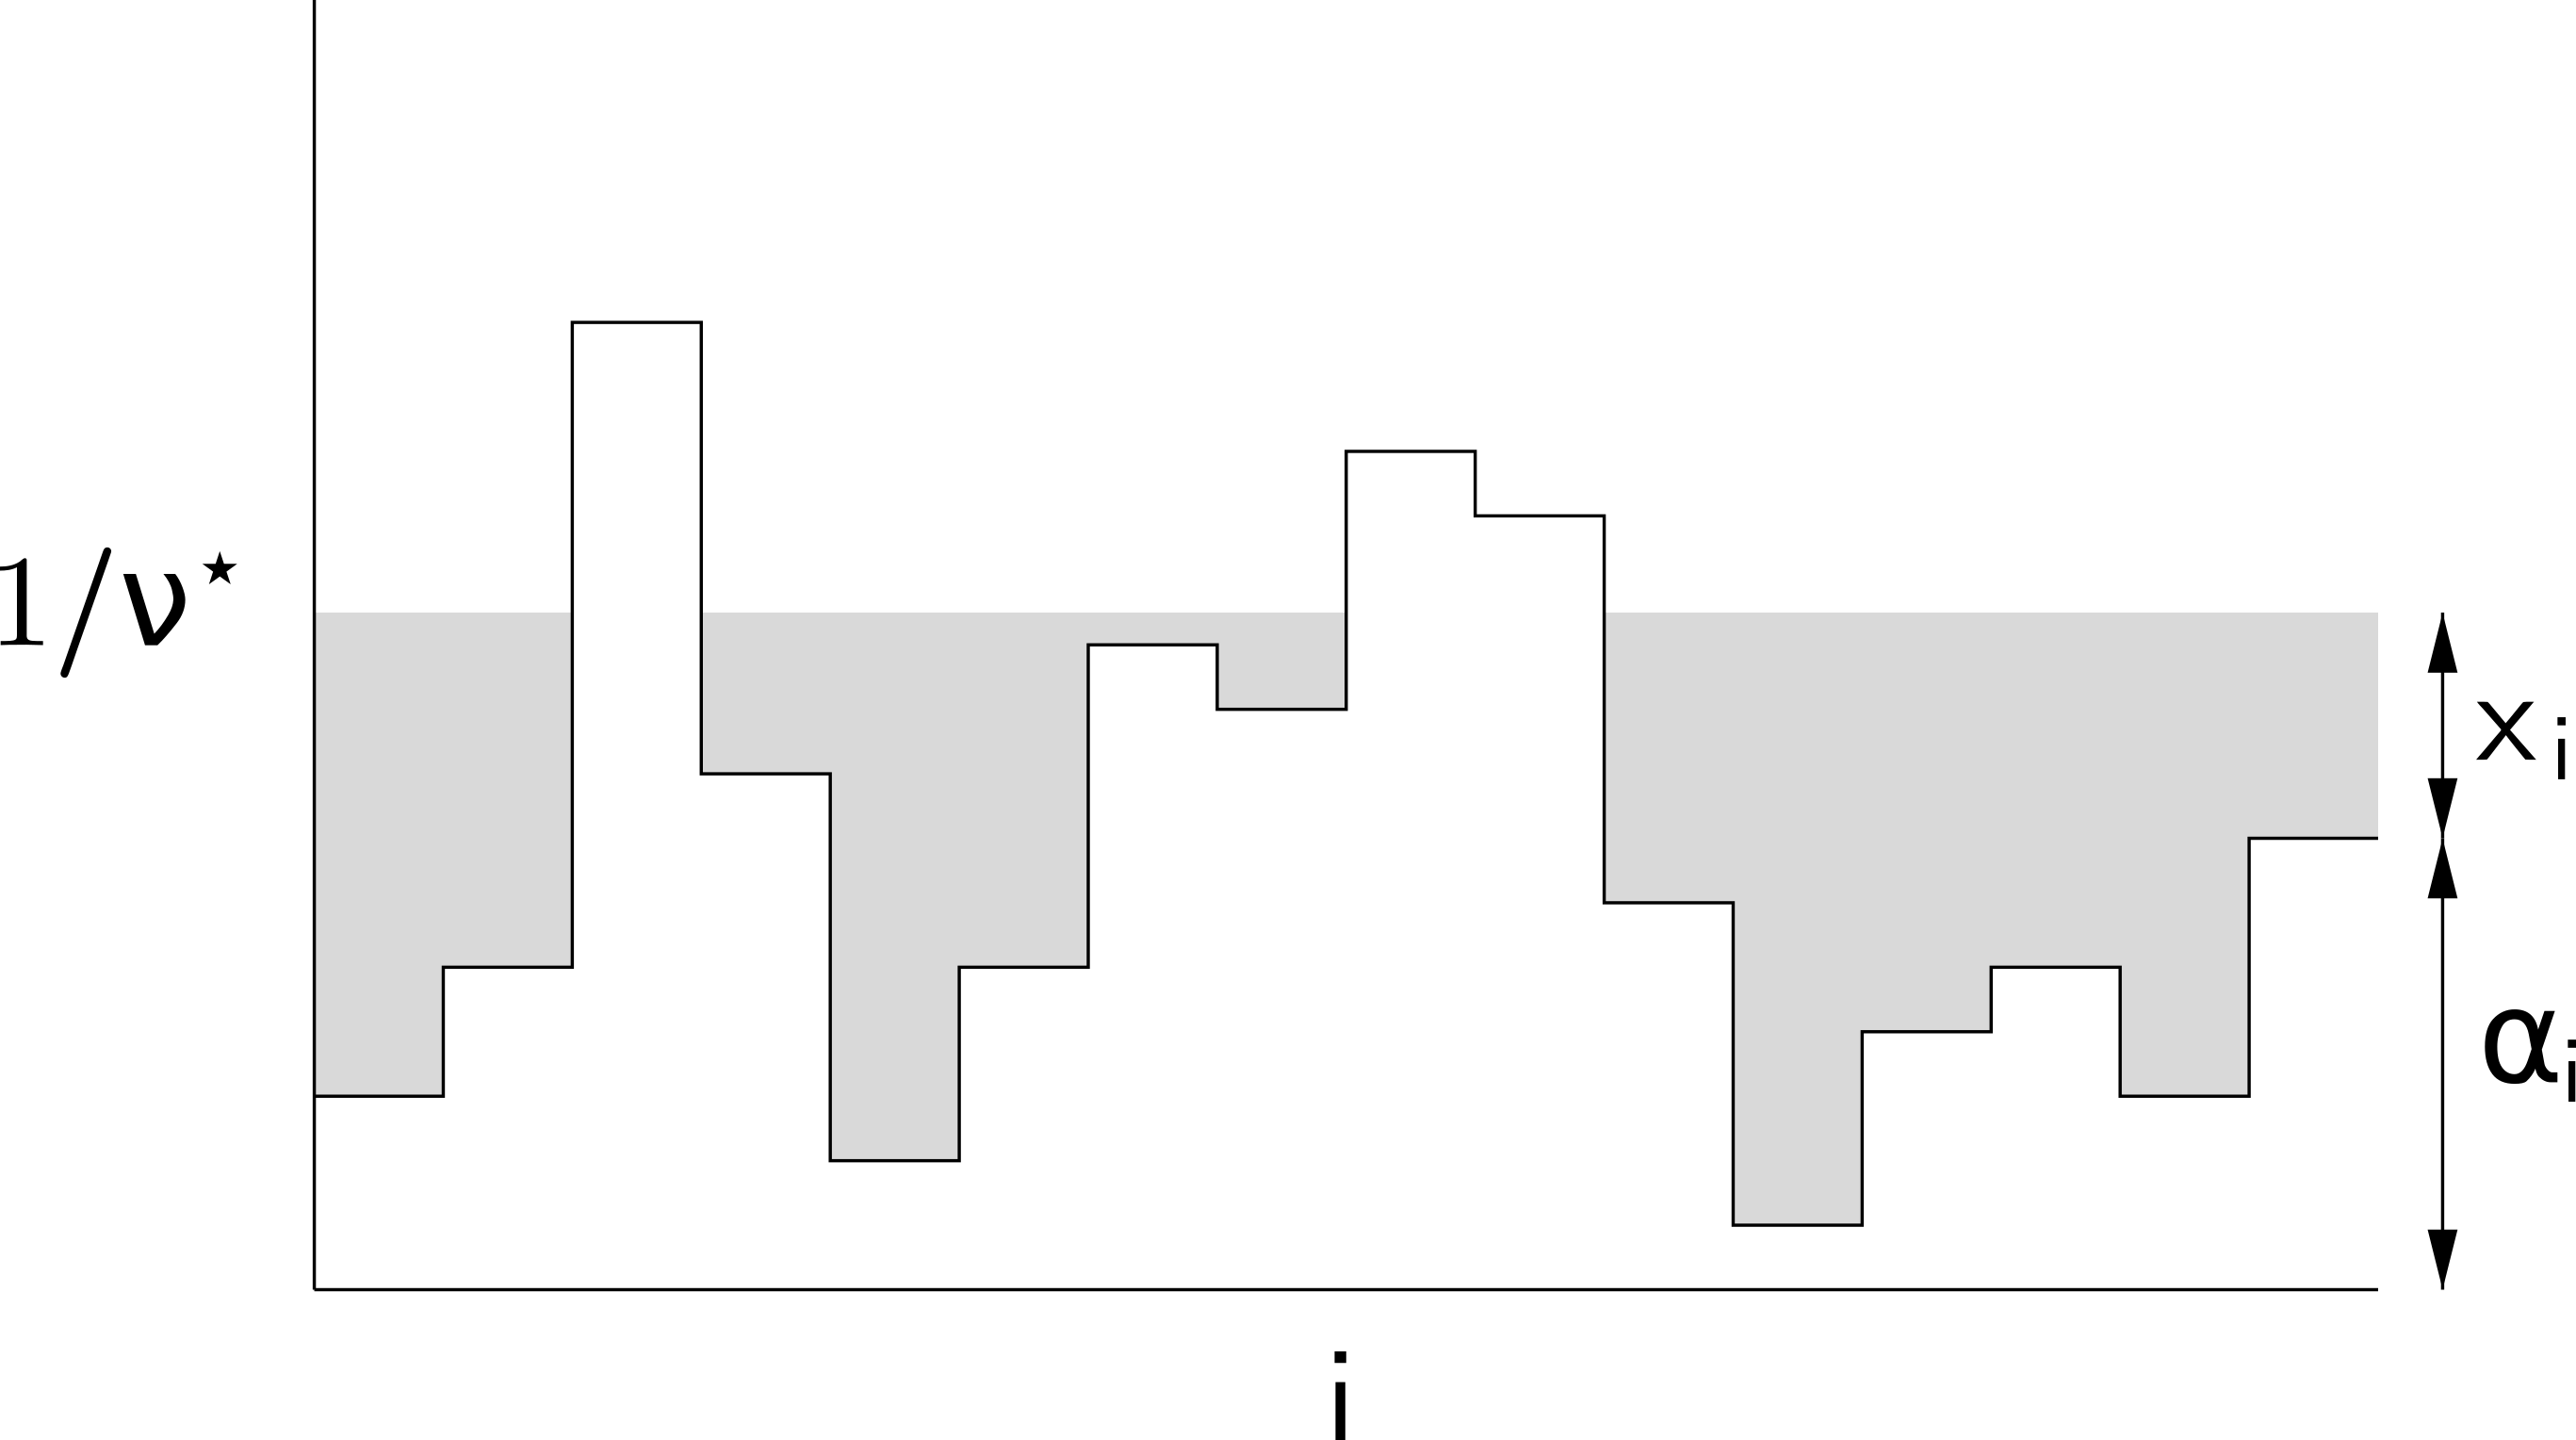
\includegraphics[width=.5\textwidth]{../Graphics/246a.png}\hfil

\clearpage
\hfil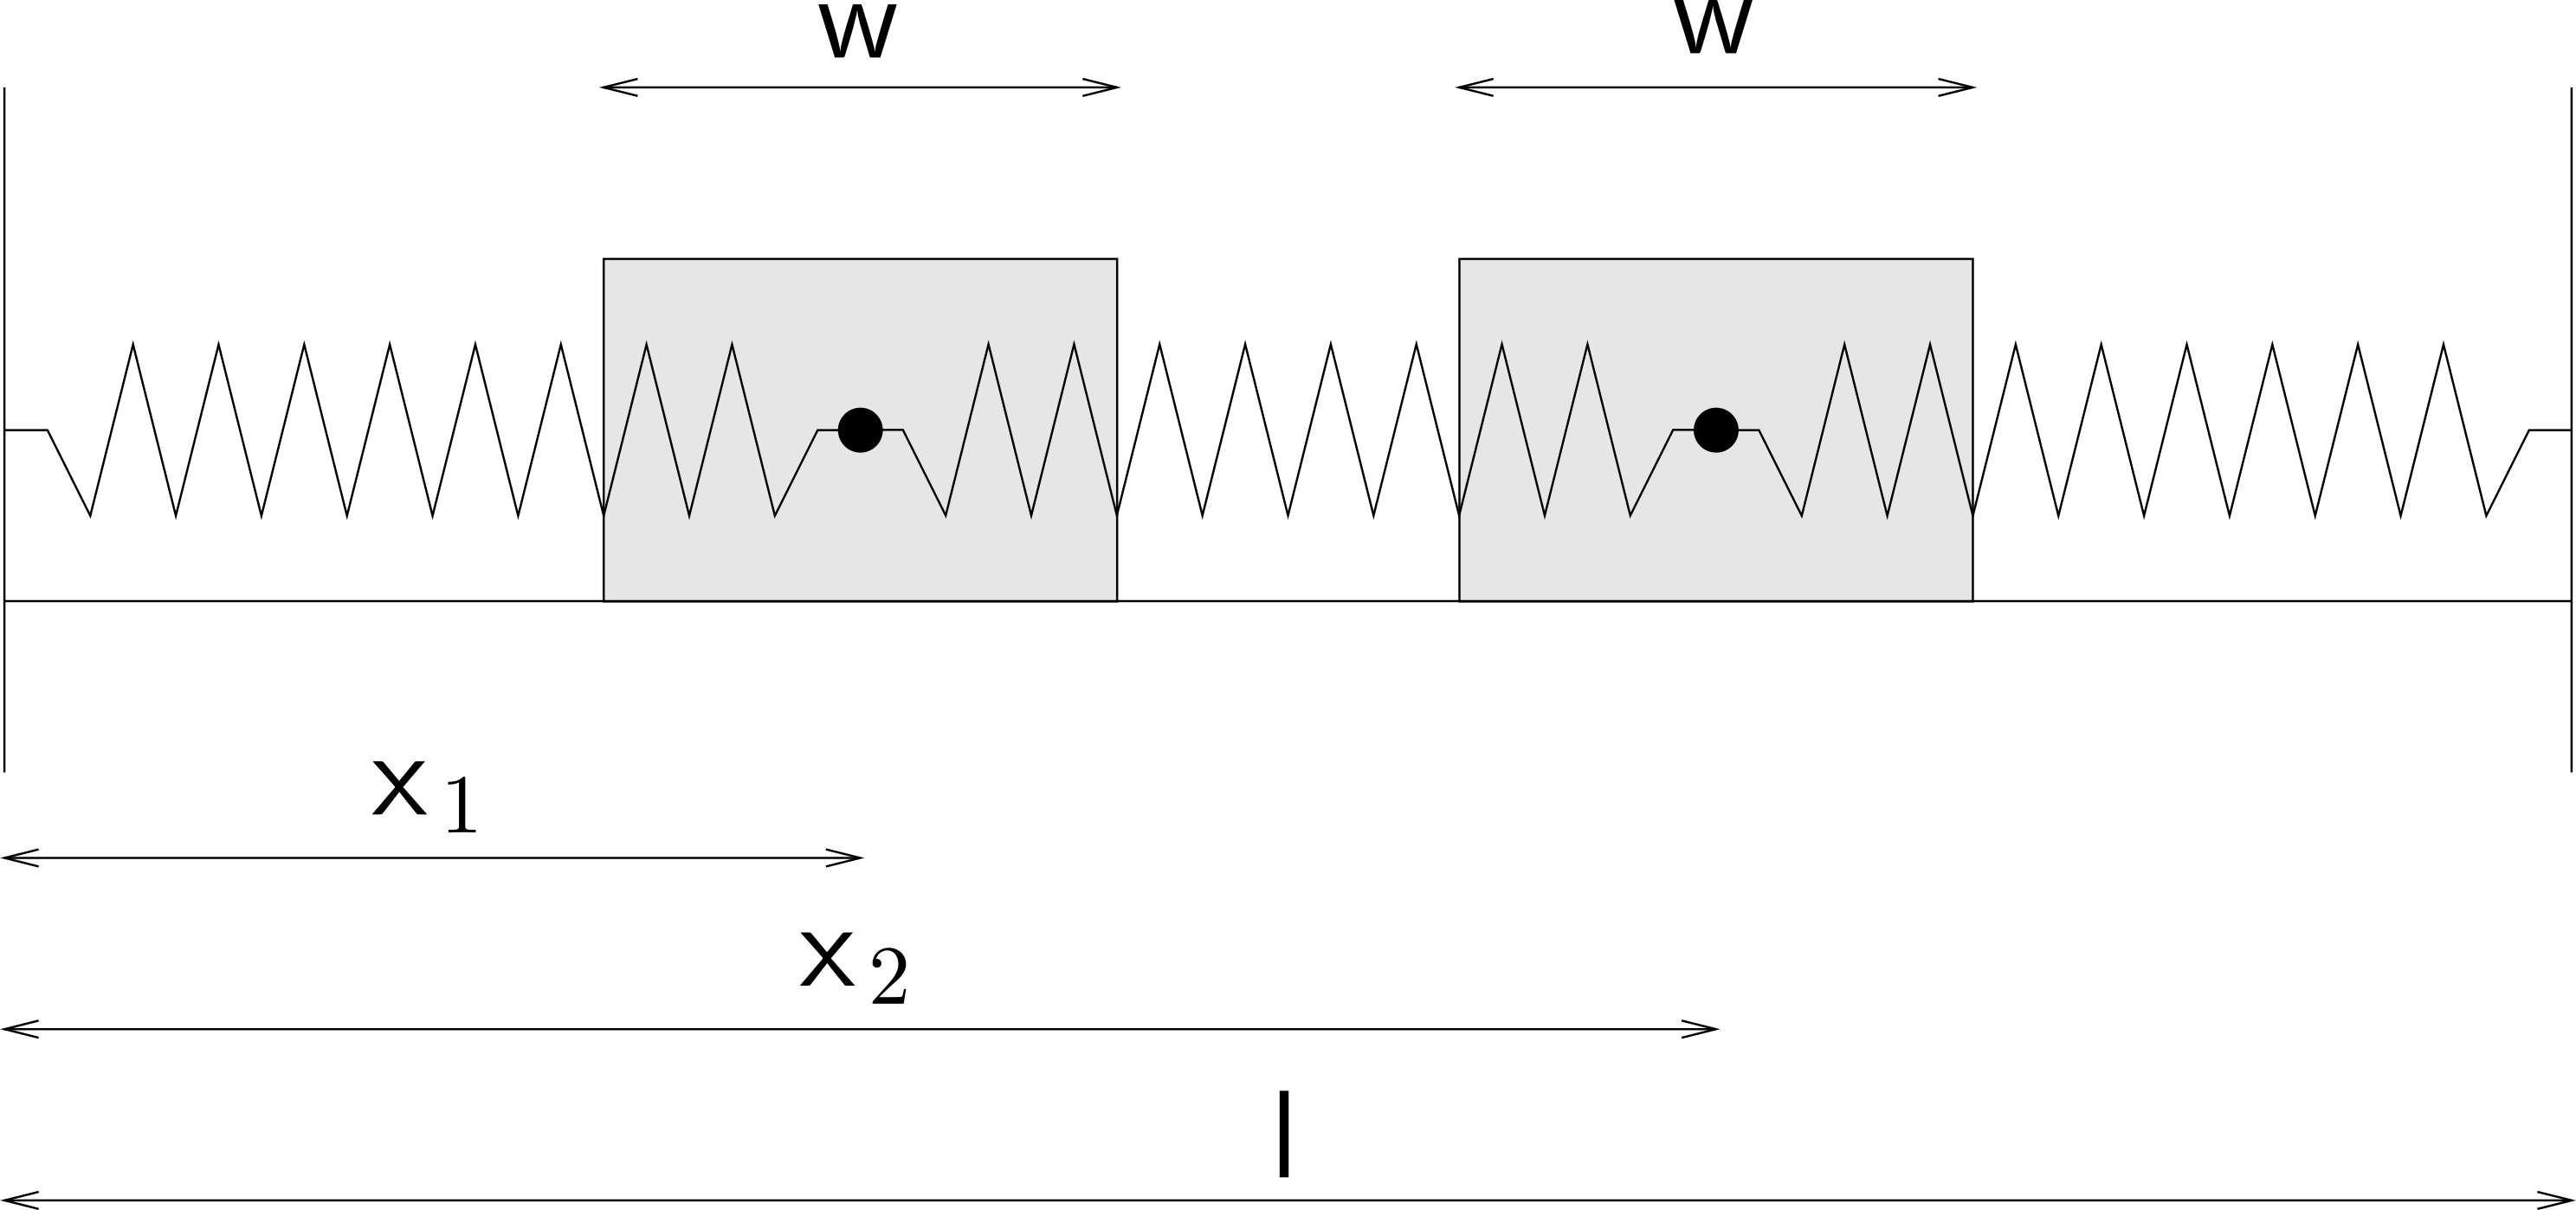
\includegraphics[width=.5\textwidth]{../Graphics/246b.png}\hfil

\clearpage
\hfil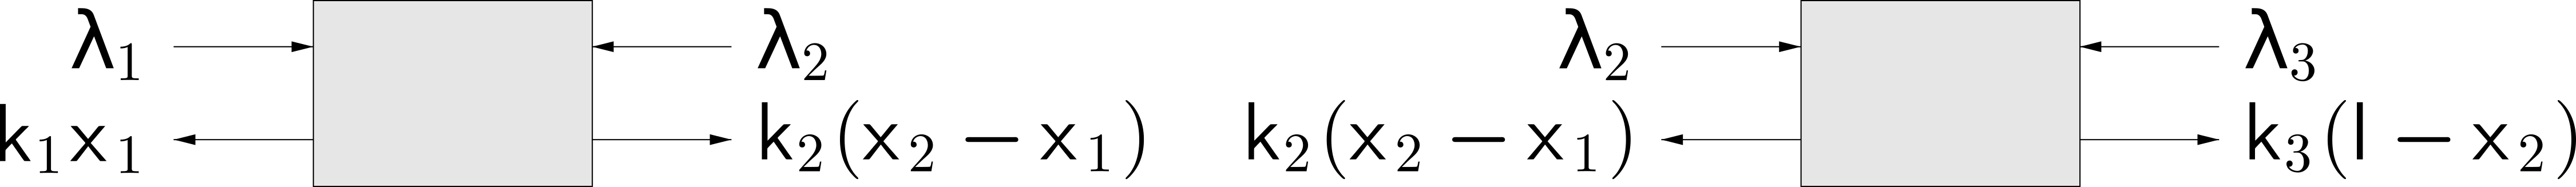
\includegraphics[width=.5\textwidth]{../Graphics/247.png}\hfil

\clearpage
\hfil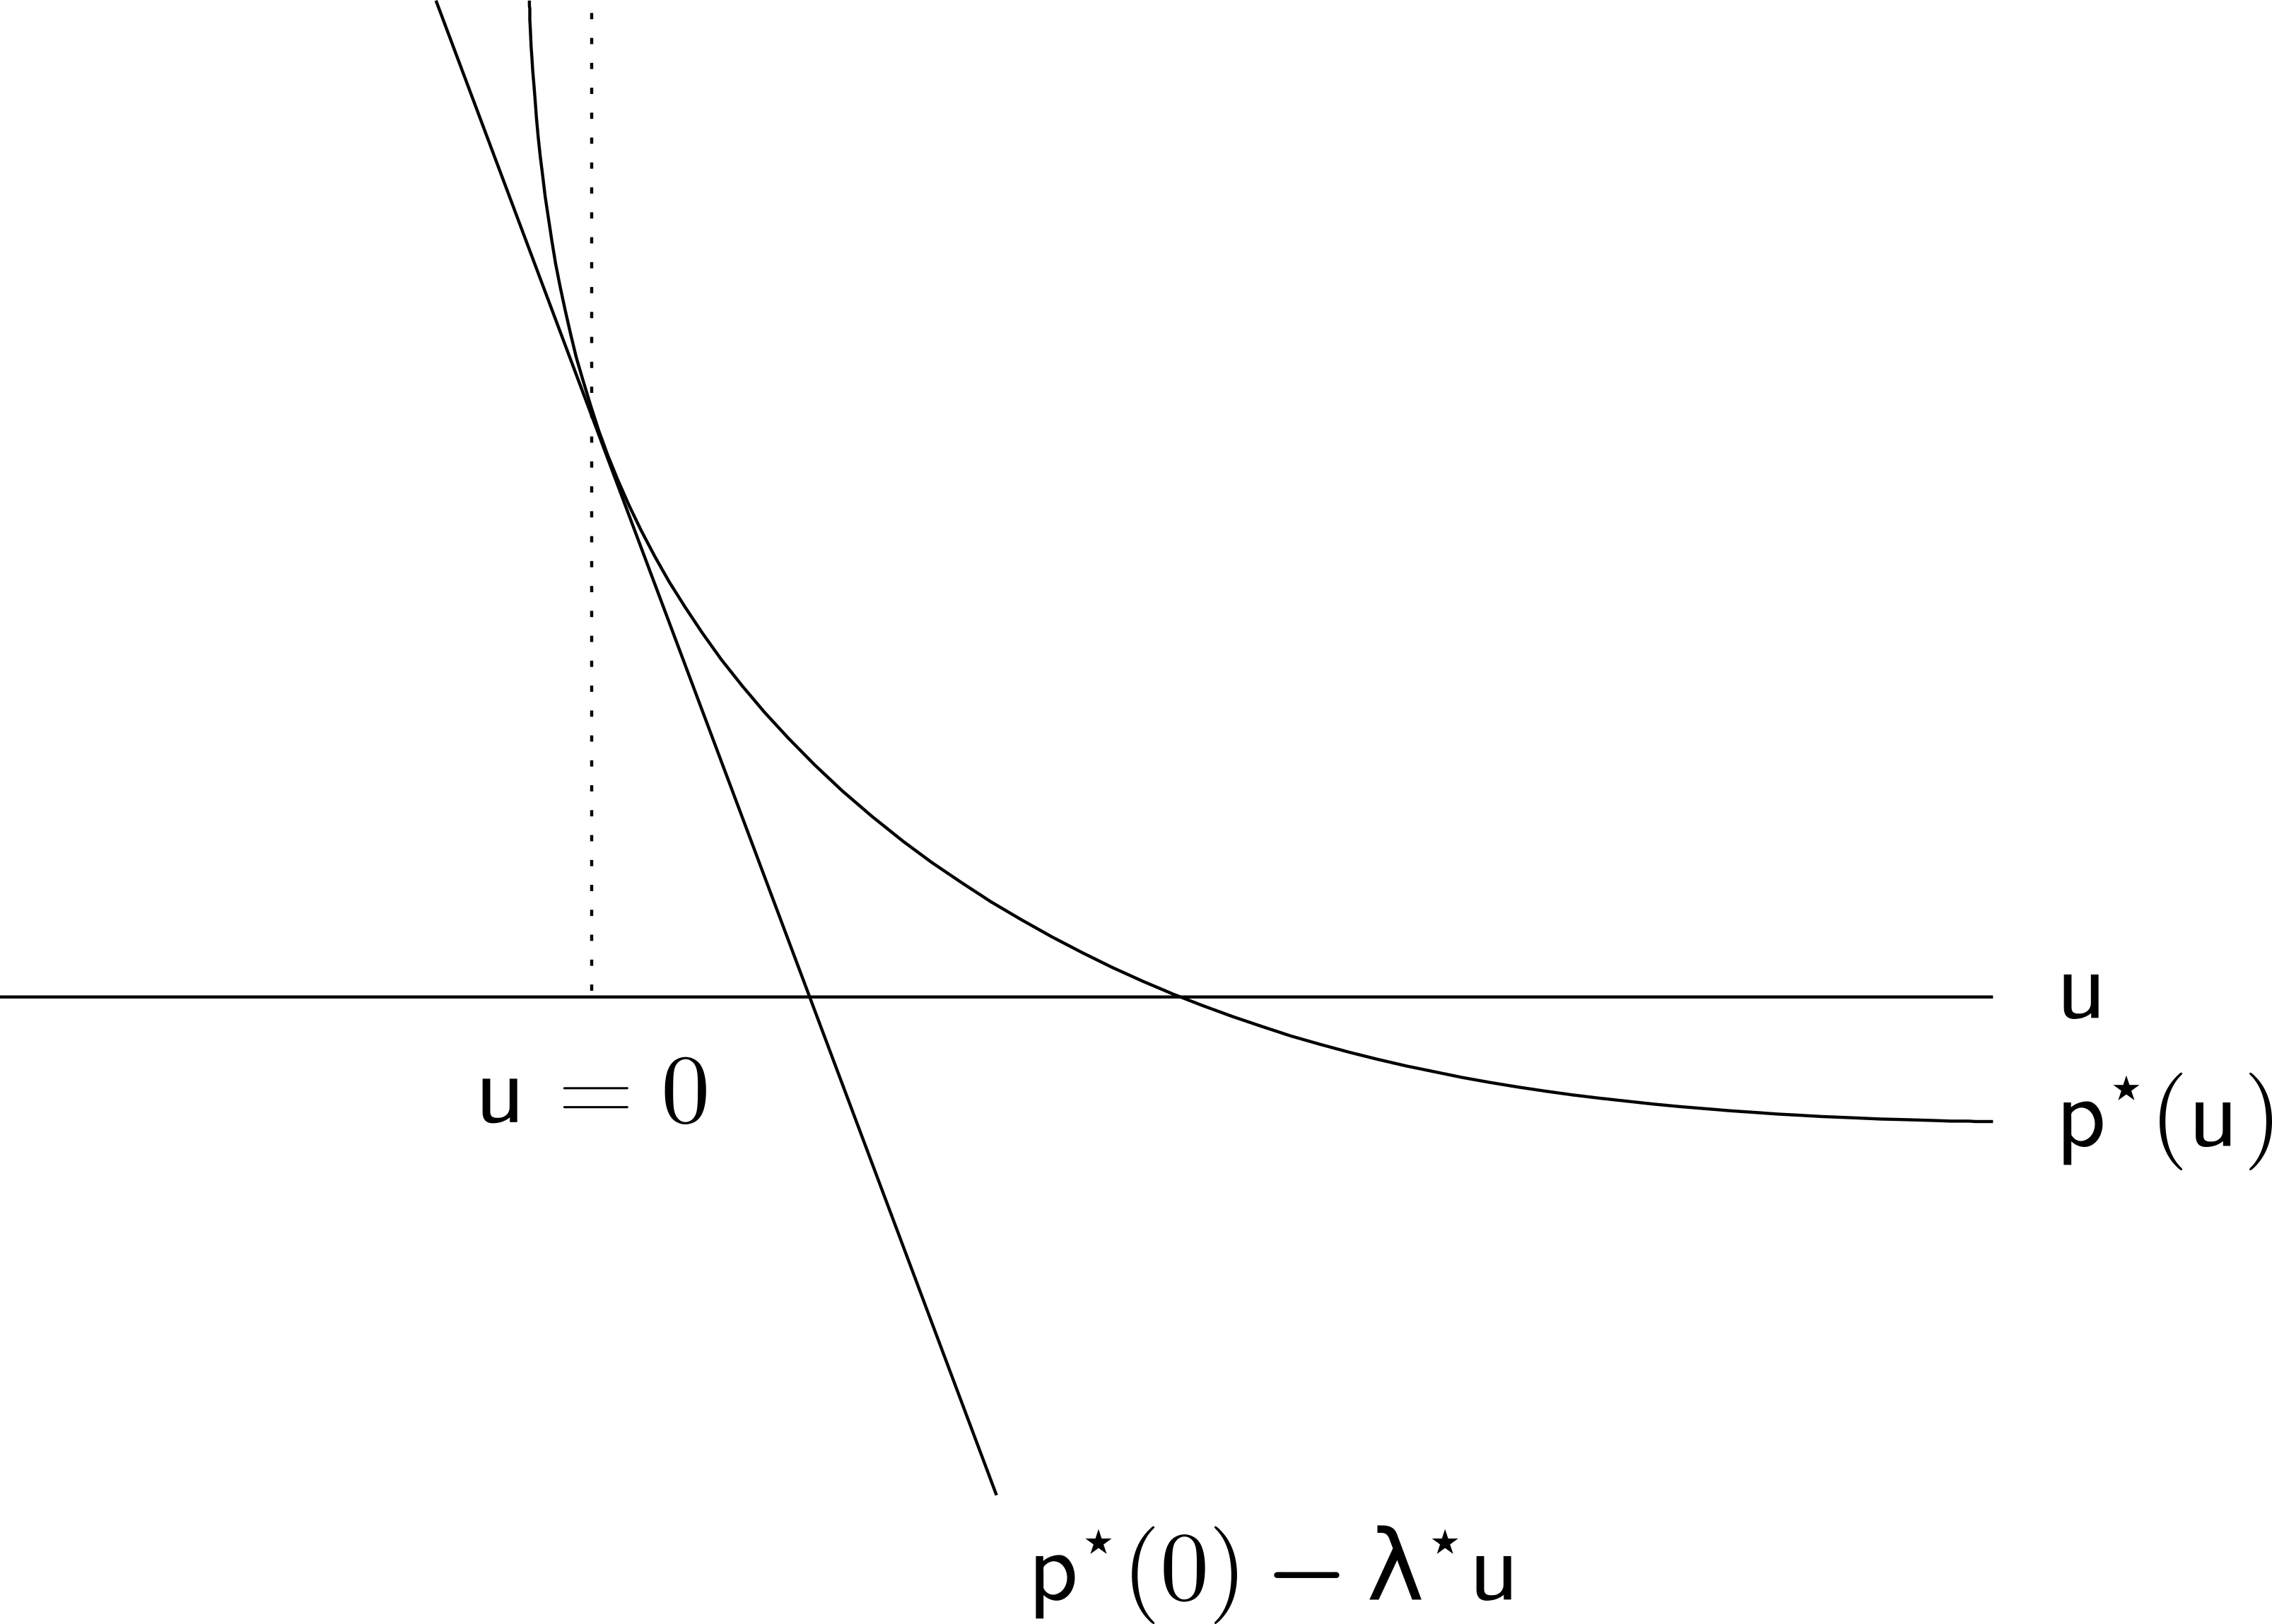
\includegraphics[width=.5\textwidth]{../Graphics/251.png}\hfil

%%% Local Variables:
%%% mode: latex
%%% TeX-master: "../LectureNotes-Optimization"
%%% End:

